\section{Compact symmetric objects}
\begin{enumerate}
    \item Introduction to CSOs
    \item What is a CSO
    \item more on the structure of CSOs
    \item The different types of CSOs
    \item The prevalence of CSOs 
    \item CSO as candidates for UHECRs and neutrinos
    \begin{enumerate}
        
       
        \item Hillas criterion, Flux of X-ray compared to diffuse flux of UHECRs and neutrinos 
        \item Kinetic jet power
        \item Timescale analysis
    \end{enumerate}
\end{enumerate}

\subsection*{Introduction to CSOs}
In regards to other types of AGN CSO or Compact symmetric objects are similar to Seyfert Galaxies. They are characterized by their small projected size 
which in \cite{kiehlmann2023compact} is described by being less than one kiloparsec and having symmetric radio emissions on both sides of the central activity. They are also in the group
of Jetted AGN, but are distinguish from other sources of jetted AGN because the jet is non-relativistic, and there is a lack of relativistic boosting. In the paper and subsequent 
papers by \cite{kiehlmann2023compact} and their group there were some overlap in classification of some sources, were some sources were classified as CSOs when in relaity they were not. 
This was due to the fact that one overlooked two "new" properties of AGN that will also be important in this paper. CSOs are also characterized by low variability in radio and low 
apparent speed along the jet. 

\subsection{Structure of CSOs}
This section will try to constate the structure of CSOs. 




\subsubsection*{Total energy density}
The total energy density of the photon fields as a function of distance is then seen in figure \ref{fig:photon_fields}. 
Here one can see that the energy density of the photon fields is constant until the observer is outside the size of the respective regions. 
From the image it is clear that the biggest contributor to the total energy density becomes the IR torus, but all the regions contribute significantly to the total energy density.

\subsubsection*{Spectral energy density}
The spectral energy density of the different regions is of more interest since this is what will determine the effect of pion decay on protons accelerate in the jet or in the lobes. To create the 
SED one has estimated the dynamical scale of our system and used the total photon densities to scale the SED accordingly. The resulting SED is seen in figure \ref{fig:SED_sep}. The SED are determined also on a number of 
parameters, all which have taken from the literature. They are seen in table \ref{tab:SED_params}.

The choice of variables comes from three sources. \cite{bronzini2024investigating} and \cite{kiehlmann2023compact} which both gives the disk luminosity of CSOs sources, and which we set to $10^{43} erg/s$. \cite{Ghisellini_2009} gives the rest of parameters that relate the different regions to the disk luminosity. The biggest caveat here is that these parameters are not specific to CSOs, but to Blazars in which they are based. For the purposes of this analysis one assumes that the parameters are the same for CSOs as for Blazars, and that one would not expect any significant difference. 

\begin{table}
    \centering
    \begin{tabular}{|c|c|}
        \hline
        Parameter & Value \\
        \hline
        $L_{d}$ & $10^{43}$ erg/s \\
        $GM$ & $G 10^{8} M_{\odot}$ \\
        $RS$ & $\frac{2GM}{c^2}$ \\
        $\eta$ & 0.1 \\
        $f_{X}$ & 0.3 \\
        $R_{X}$ & 30$ RS $\\
        $\beta$ & 0.4 $c$\\
        $f_{\text{BLR}}$ & 0.1 \\
        $R_{\text{BLR}}$ & $10^{17} \sqrt{L_{d}/10^{45}}$ cm \\
        $f_{\text{IR}}$ & 0.5 \\
        $R_{\text{IR}}$ & $2.5 10^{18}\sqrt{L_{d}/10^{45}}$ cm \\
        $\Gamma$ & 1.1 \\
        \hline
    \end{tabular}
    \caption{Parameters used to determine the SED of the different regions.}
    \label{tab:SED_params}
\end{table}
\begin{figure}
    \centering
    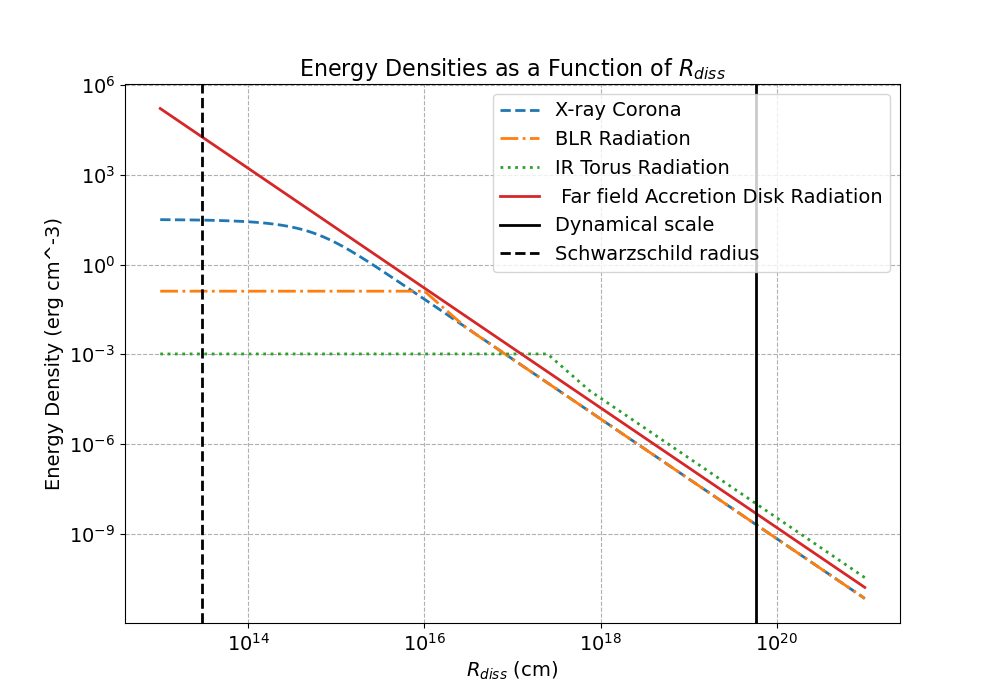
\includegraphics[width=.5\textwidth]{C:/Users/henri/OneDrive/Documents/NTNU/Semester 10/Masteroppgave/Plots/Energy_densities.png}
    \caption{The total energy density of the photon fields as a function radius from central engine.}
    \label{fig:photon_fields}
\end{figure}


\begin{figure}
    \centering
    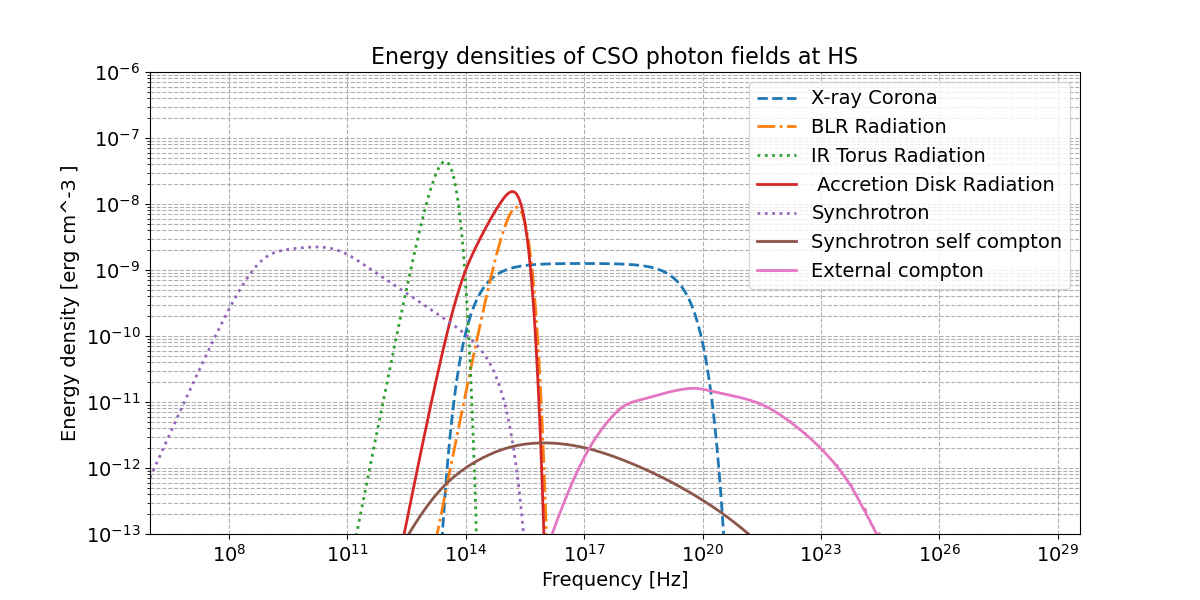
\includegraphics[width=.5\textwidth]{C:/Users/henri/OneDrive/Documents/NTNU/Semester 10/Masteroppgave/Plots/SEDs_sep.png}
    \caption{The spectral energy density at distance R}
    \label{fig:SED_sep}
\end{figure}

\begin{figure}
    \centering
    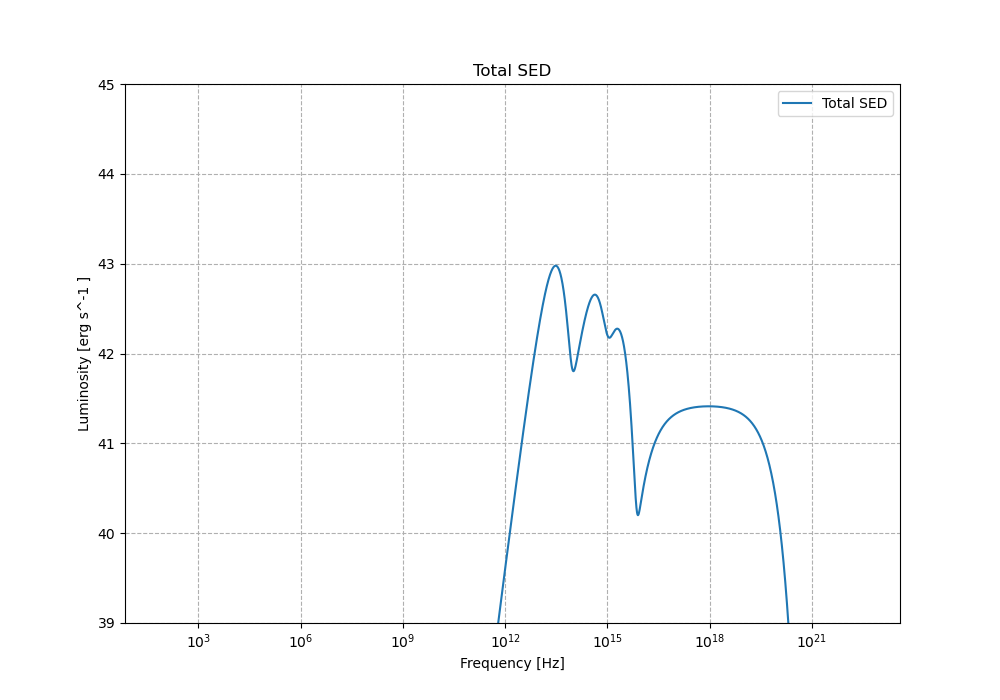
\includegraphics[width=.5\textwidth]{C:/Users/henri/OneDrive/Documents/NTNU/Semester 10/Masteroppgave/Plots/SED.png}
    \caption{Luminosity of the different components of the CSO that are close by the central engine. Missing synchrotron and IC part which is most prominent }
    \label{fig:Lum_SED}
\end{figure}

\subsection{Classification of CSO}
From the papers of \cite{kiehlmann2023compact} to \cite{readhead2023compact}, and from \cite{sullivan2024smallscale} there is a clear quite new classification of CSOs. The classification is based on firstly CSOs being edge brightened or edge dimmed. Edge brightened sources which will onwards be refered as CSO 2s are bright in radio in their lobes, and CSO 1s or edge dimmed are thought to be CSOs that have stalled. 

The big picture on CSOs is that they are a group of very short-lived sources that are ignited by transient events. Saying if the ignition of their jets are due to transient event such as tidal disruption event are covered in \cite{sullivan2024smallscale} and for the purposes of this study not necessary to discuss, but start a very interesting conversation. CSOs are then symmetric with the expansion of their jets into the interstellar medium visible from radio telescope. The symmetry of the jets is a key feature of CSOs and makes them unique in the sense of jetted-AGN since they have little to no features of relativistic beaming.   


\subsection{Catalouge of Bona fide CSO}
In order to study these sources there will always be a need for observational data. This fact combined with the fact that CSOs are a somewhat new class of AGN mean that there are no large catalogues of pure CSOs, and that many other catalogues misnomer sources as CSOs. This chapter will rely heavilly on \cite{kiehlmann2023compact} in which this is discussed and where they define a bona fide catalogue of 79 CSOs. The catalogue will allow us as it has in this paper to say more concrete infromation about the sources we are studying.



\subsection{Prevalence of CSOs}







\subsection{Stability in jet expansion and lobes.} The most promesing feature of CSOs which we will see as a key feature in the section on time-scales is the stability of the lobes in radio emission, the stability of the jet expansion and the stability of most wavelengths in emissions. In \cite{bronzini2024investigating} they report no significant variablilty of one CSO source in gamma rays, variability of the order of years in x-ray, with the broadband SED showing variability on the timescales of years. This is a clear distincsion from other jetted AGN which are known to be highly variable. Having stable systems allows for more efficient acceleration of ions, and significantly increases the possibility of producing UHECRs. 